
\documentclass[tikz,convert={convertexe={magick.exe}}]{standalone}
\usetikzlibrary{patterns}
\begin{document}
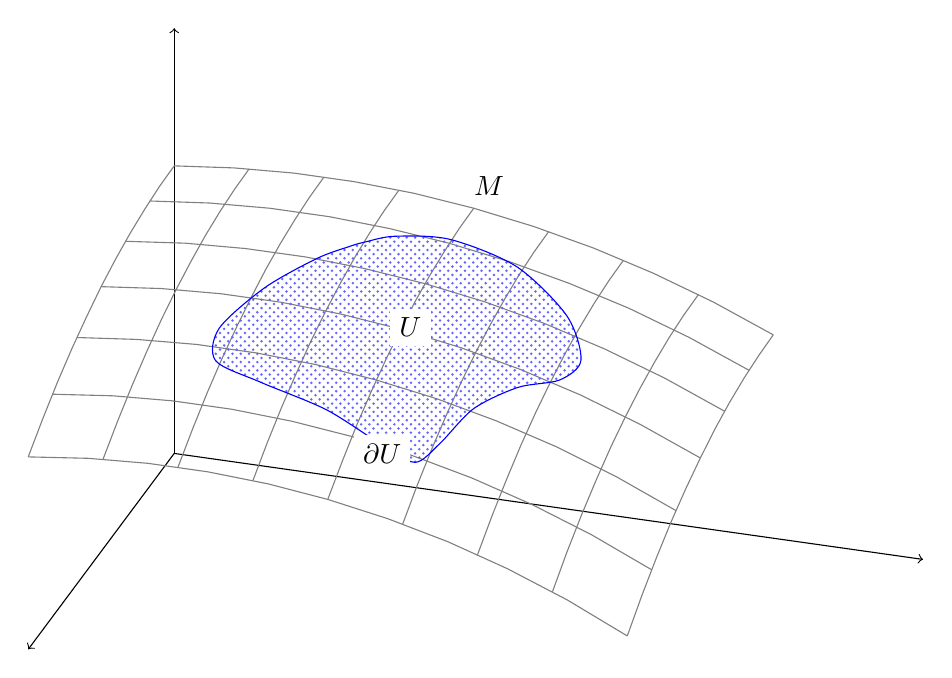
\begin{tikzpicture}[scale=2]
\draw[->] (0.000,0.000)--(-0.927,-1.244);
\draw[->] (0.000,0.000)--(4.755,-0.673);
\draw[->] (0.000,0.000)--(0.000,2.700);
\draw[gray] (0.000,1.826)--(0.380,1.813)--(0.761,1.780)--(1.141,1.726)--(1.522,1.652)--(1.902,1.557)--(2.283,1.441)--(2.663,1.304)--(3.043,1.144)--(3.424,0.961)--(3.804,0.753);
\draw[gray] (-0.155,1.603)--(0.226,1.590)--(0.606,1.557)--(0.987,1.503)--(1.367,1.428)--(1.748,1.334)--(2.128,1.218)--(2.508,1.080)--(2.889,0.921)--(3.269,0.737)--(3.650,0.528);
\draw[gray] (-0.309,1.347)--(0.071,1.335)--(0.452,1.301)--(0.832,1.248)--(1.213,1.173)--(1.593,1.078)--(1.974,0.962)--(2.354,0.824)--(2.734,0.663)--(3.115,0.478)--(3.495,0.268);
\draw[gray] (-0.464,1.059)--(-0.083,1.047)--(0.297,1.014)--(0.678,0.960)--(1.058,0.885)--(1.439,0.789)--(1.819,0.672)--(2.199,0.533)--(2.580,0.371)--(2.960,0.184)--(3.341,-0.029);
\draw[gray] (-0.618,0.736)--(-0.238,0.724)--(0.143,0.692)--(0.523,0.638)--(0.904,0.563)--(1.284,0.466)--(1.665,0.348)--(2.045,0.207)--(2.425,0.043)--(2.806,-0.147)--(3.186,-0.363);
\draw[gray] (-0.773,0.376)--(-0.392,0.366)--(-0.012,0.334)--(0.369,0.280)--(0.749,0.204)--(1.130,0.107)--(1.510,-0.013)--(1.890,-0.156)--(2.271,-0.324)--(2.651,-0.517)--(3.032,-0.739);
\draw[gray] (-0.927,-0.022)--(-0.547,-0.031)--(-0.166,-0.063)--(0.214,-0.117)--(0.595,-0.193)--(0.975,-0.292)--(1.355,-0.414)--(1.736,-0.560)--(2.116,-0.732)--(2.497,-0.931)--(2.877,-1.159);
\draw[gray] (0.000,1.826)--(-0.093,1.696)--(-0.185,1.554)--(-0.278,1.401)--(-0.371,1.236)--(-0.464,1.059)--(-0.556,0.869)--(-0.649,0.667)--(-0.742,0.451)--(-0.834,0.222)--(-0.927,-0.022);
\draw[gray] (0.476,1.807)--(0.383,1.677)--(0.290,1.535)--(0.197,1.382)--(0.105,1.217)--(0.012,1.040)--(-0.081,0.851)--(-0.173,0.650)--(-0.266,0.435)--(-0.359,0.206)--(-0.452,-0.037);
\draw[gray] (0.951,1.755)--(0.858,1.625)--(0.766,1.484)--(0.673,1.331)--(0.580,1.166)--(0.488,0.989)--(0.395,0.800)--(0.302,0.599)--(0.209,0.384)--(0.117,0.156)--(0.024,-0.087);
\draw[gray] (1.427,1.672)--(1.334,1.542)--(1.241,1.400)--(1.148,1.247)--(1.056,1.082)--(0.963,0.906)--(0.870,0.717)--(0.778,0.515)--(0.685,0.300)--(0.592,0.071)--(0.500,-0.172);
\draw[gray] (1.902,1.557)--(1.809,1.427)--(1.717,1.285)--(1.624,1.132)--(1.531,0.967)--(1.439,0.789)--(1.346,0.600)--(1.253,0.397)--(1.160,0.182)--(1.068,-0.048)--(0.975,-0.292);
\draw[gray] (2.378,1.409)--(2.285,1.279)--(2.192,1.137)--(2.100,0.983)--(2.007,0.817)--(1.914,0.640)--(1.821,0.449)--(1.729,0.246)--(1.636,0.029)--(1.543,-0.202)--(1.451,-0.448);
\draw[gray] (2.853,1.227)--(2.760,1.097)--(2.668,0.955)--(2.575,0.800)--(2.482,0.634)--(2.390,0.455)--(2.297,0.263)--(2.204,0.058)--(2.112,-0.161)--(2.019,-0.394)--(1.926,-0.643);
\draw[gray] (3.329,1.009)--(3.236,0.879)--(3.143,0.736)--(3.051,0.581)--(2.958,0.414)--(2.865,0.233)--(2.772,0.040)--(2.680,-0.168)--(2.587,-0.389)--(2.494,-0.626)--(2.402,-0.878);
\draw[gray] (3.804,0.753)--(3.712,0.622)--(3.619,0.479)--(3.526,0.323)--(3.433,0.154)--(3.341,-0.029)--(3.248,-0.225)--(3.155,-0.435)--(3.063,-0.660)--(2.970,-0.901)--(2.877,-1.159);

\draw[blue, pattern=crosshatch dots, pattern color=blue!60] plot[smooth] coordinates{(1.320,0.050) (1.529,-0.057) (1.688,0.064) (1.901,0.284) (2.182,0.419) (2.449,0.467) (2.583,0.592) (2.493,0.874) (2.176,1.185) (1.752,1.359) (1.401,1.379) (1.214,1.343) (1.103,1.311) (0.902,1.236) (0.573,1.051) (0.286,0.795) (0.263,0.589) (0.549,0.452) (0.971,0.275) (1.320,0.050)};

\node[fill=white] at (1.5,.8) {$U$};

\node[fill=white] at (1.320,0) {$\partial U$};

\node at (2,1.7) {$M$};

\end{tikzpicture}
\end{document}